\documentclass[10pt,conference]{IEEEtran}
\IEEEoverridecommandlockouts
\usepackage{cite}
\usepackage{amsmath}
\usepackage{booktabs}
\usepackage{xcolor}
\usepackage{tikz}
\usetikzlibrary{arrows.meta,positioning,fit,calc}
\usepackage{url}
\usepackage[hidelinks]{hyperref}
\usepackage{listings}
\lstset{basicstyle=\ttfamily\tiny,columns=fullflexible,frame=single,framesep=2pt,xleftmargin=3pt,xrightmargin=3pt,aboveskip=4pt,belowskip=2pt,belowcaptionskip=4pt,
  literate={·}{{$\cdot$}}1 {→}{{$\to$}}1 {—}{{\textemdash}}1}

\newcommand{\tool}{Git4agents}

\begin{document}

\title{\tool{}: Governed Promotion and Conflict Resolution for Fleets of Coding Agents}

\author{\IEEEauthorblockN{Yashwanth Gathuku}
\IEEEauthorblockA{Independent researcher, Cleveland, Ohio, USA\\
yashwanth8035@gmail.com}}

\maketitle

\begin{abstract}
Coding agents now work on one repository in parallel, and Git is a poor gatekeeper for them: it records ancestry, but a passing CI run, a branch permission or a clean merge says little about whether an agent's state should become canonical, and overlapping edits are left to people. \tool{} keeps Git as the history layer and governs canonicalization around it. Agents write only to isolated contender forks under declared work claims; an independent evaluator, blind commit-then-reveal verifiers and non-compensatory gates decide; a single-use permit bound to the exact reviewed commit authorizes promotion; and every promotion ships a signed bundle that verifies offline. This demonstration adds \emph{governed resolution}: when agents edit the same lines, an untrusted resolver may write only the conflicted hunks, each agent's frozen witness checks must still pass, and the resolved commit is bound to a content-addressed conflict capsule in the signed ledger. In 64 resolution attempts on eight conflicting scenarios over three npm packages, the earlier resolve path admitted 37 wrong resolutions; the governed path admitted none and refused one correct one. \tool{} runs on Cloudflare Workers, Durable Objects and Artifacts.
Code and a ready-to-run container: \url{https://github.com/YashwanthGathuku/Git4agents/tree/icse27-tool-paper}. Video: \url{https://youtu.be/VIDEO-ID}
\end{abstract}

\section{Introduction}
Concurrent coding agents collide often. Merge simulation of more than 107,000 agent pull requests found conflicts in 27.7\% of them~\cite{ogenrwot2026agenticflict}. Replaying merges of 747 pairs of co-active pull requests, Xu et al.\ found textual conflicts in 41.7\% of cross-agent pairs against 19.8\% of pairs by the same agent~\cite{xu2026agentprs}. Handing those conflicts to a language model is not yet a safe default. The best models reproduce fewer than 60\% of developers' resolutions~\cite{schesch2026mergebench}; high textual similarity to the developer's file does not mean a resolution is safe~\cite{zhang2026swegitbench}; and an LLM judge accepted four of five structurally invalid resolutions~\cite{shen2026llmjudge}.

Git's governance assumes a few people who take turns: branch permissions decide who may merge, CI trusts the tests in the branch, and the merge itself is the record. With agent fleets each assumption fails. An agent can claim a task is done when it is not, edit the tests it is judged by, push stale state, or resolve a conflict by quietly keeping one side. \tool{} separates the two questions Git conflates: \emph{Git decides ancestry; \tool{} decides canonicality.} This paper contributes:
\begin{itemize}
\item a deployed trust layer that admits agent work to canonical history only through independent evidence, non-overridable gates and an exact-state, single-use permit, with offline-verifiable proof (Sec.~\ref{sec:tool});
\item \emph{governed resolution}: a hunk-level resolution lease, frozen per-agent witness checks, a resolution ladder whose model rung must agree in both orders, and a binding of every resolved commit to its conflict capsule (Sec.~\ref{sec:resolution});
\item evidence from live runs on Cloudflare and a resolution benchmark of 204 attempts (Sec.~\ref{sec:eval}).
\end{itemize}

\section{The \tool{} Trust Layer}\label{sec:tool}
\tool{} is one Cloudflare Worker. A \emph{TaskAuthority} Durable Object per task is the single writer of its state: the frozen task and baseline, work claims, conflict reports, contenders, evaluations, verifier commitments, verdicts, permits and a hash-chained ledger. Cloudflare Artifacts~\cite{cf-artifacts} holds the canonical repository and one fork per contender; push events reach the authority through a Queue; a Workflow and a Container perform the only canonical write. Control, agent and evaluation calls use separate credentials.

Fig.~\ref{fig:flow} shows a task's path. Agents first declare \emph{WorkClaims}---paths, symbols, contracts read and modified---which deterministic set rules classify as GREEN, AMBER, RED or BLOCKED. Each contender commits to its own fork; a \emph{fork crew} of sub-agents shares one fork, and per-file three-way merges compose their commits into one candidate or report a conflict. An independent evaluator runs hidden tests against the immutable candidate; editing test files or runner configuration is evidence tampering and quarantines the contender mechanically. Blind verifiers commit to SHA-256 commitments before they see candidates and then reveal. The verdict seam evaluates mandatory gates first and never lets a score compensate for a failed gate; no override path exists. On ACCEPT the authority issues a permit whose id hashes the task, baseline, candidate tree, evidence, policy and expected destination head. It is single-use and expires if the destination head moves. Promotion fast-forwards to the reviewed commit itself, and the authority signs in-toto statements~\cite{torresarias2019intoto} in DSSE envelopes~\cite{dsse} together with the ledger, which anyone can check offline against a pinned key.

Agents reach \tool{} over REST or the Model Context Protocol~\cite{mcp}. The MCP surface has seven tools---inspect the task and work graph, check clearance, claim work, open a contender fork, read the ledger, verify a permit---and deliberately none that evaluates, decides, issues a permit or promotes.

\begin{figure*}[t]
\centering
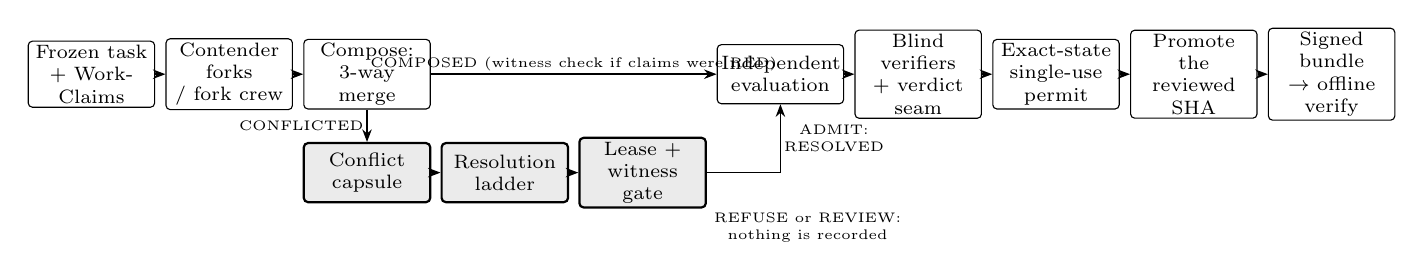
\begin{tikzpicture}[
  font=\scriptsize, x=17.5mm, y=10mm,
  box/.style={draw, rounded corners=1.5pt, align=center, inner sep=1.5pt, minimum height=7.5mm, text width=15mm},
  gov/.style={box, fill=black!8, thick},
  arr/.style={-{Stealth[length=1.6mm]}, semithick},
  lab/.style={font=\tiny, inner sep=1pt, align=center}]
\node[box] (task) at (0,0) {Frozen task\\+ WorkClaims};
\node[box] (forks) at (1,0) {Contender forks\\/ fork crew};
\node[box] (compose) at (2,0) {Compose:\\3-way merge};
\node[box] (eval) at (5,0) {Independent\\evaluation};
\node[box] (verdict) at (6,0) {Blind verifiers\\+ verdict seam};
\node[box] (permit) at (7,0) {Exact-state\\single-use permit};
\node[box] (promote) at (8,0) {Promote the\\reviewed SHA};
\node[box] (bundle) at (9,0) {Signed bundle\\$\to$ offline verify};
\node[gov] (capsule) at (2,-1.25) {Conflict\\capsule};
\node[gov] (ladder) at (3,-1.25) {Resolution\\ladder};
\node[gov] (gate) at (4,-1.25) {Lease +\\witness gate};
\draw[arr] (task) -- (forks);
\draw[arr] (forks) -- (compose);
\draw[arr] (compose) -- node[lab, above] {COMPOSED (witness check if claims were RED)} (eval);
\draw[arr] (compose) -- node[lab, left] {CONFLICTED} (capsule);
\draw[arr] (capsule) -- (ladder);
\draw[arr] (ladder) -- (gate);
\draw[arr] (gate.east) -| node[lab, right, pos=0.75] {ADMIT:\\RESOLVED} (eval.south);
\draw[arr] (eval) -- (verdict);
\draw[arr] (verdict) -- (permit);
\draw[arr] (permit) -- (promote);
\draw[arr] (promote) -- (bundle);
\node[lab, anchor=north west] at ($(gate.south east)+(0.5mm,-0.2mm)$) {REFUSE or REVIEW:\\nothing is recorded};
\end{tikzpicture}
\caption{A task in \tool{}. Shaded steps are governed resolution (Sec.~\ref{sec:resolution}): the resolution ladder tries Mergiraf, then intent replay in both orders, and every candidate must pass the hunk lease and the frozen witness gate. The task authority records every step before promotion; only the promotion path writes canonical history.}
\label{fig:flow}
\end{figure*}

\section{Governed Resolution}\label{sec:resolution}
Before this work, a conflicted crew either stopped or ran an operator's resolver command, checked only for leftover conflict markers. Auditing that path, we found that the resolver had to rebuild every clean edit itself and could write anywhere: a resolver that wrote one file produced a commit whose parents named every agent's commit while its tree held none of their other work. Governed resolution treats every resolver---a structured merge tool, a model, a person's script---as an untrusted producer.

\textbf{Resolution lease.} The authority writes the \emph{pre-composed} tree: the baseline plus every non-conflicting edit, including the clean regions of a conflicted file, which \texttt{git merge-file --diff3} splits into clean segments and conflicted hunks. Each hunk holds its baseline text. The resolver reads its inputs from outside the repository and may change only the hunks; the resolved file must contain every clean segment byte-for-byte and in order, or the resolution is refused. Files with three or more sides are leased whole.

\textbf{Conflict capsule.} A \texttt{CONFLICTED} record becomes a content-addressed capsule: digests of the baseline, contributing commits, every hunk and the frozen witness manifest. The authority computes its id itself.

\textbf{Frozen witnesses.} Each agent declares small checks of its own intent in the crew configuration. They are read and hashed once, before any agent runs, and executed from copies outside every candidate tree, so neither an agent nor a resolver can weaken them. A check $t$ counts as a witness for side $i$ only if it discriminates that side:
\begin{equation}
\mathit{witness}_i(t) \iff \lnot\mathit{pass}(t,\mathit{base}) \land \mathit{pass}(t,\mathit{sha}_i).
\end{equation}
A candidate $R$ is refused (REFUSE) if any witness fails on $R$ or a check that passed on the baseline regresses; it goes to REVIEW if some conflicting side has no witness, since absent evidence is not evidence that intent survived; otherwise it is admitted (ADMIT). SAM~\cite{dasilva2024sam} applies a similar pass/fail criterion with generated unit tests to \emph{detect} semantic conflicts after a merge; \tool{} uses agent-declared checks, frozen before an untrusted resolver runs, as a non-compensatory \emph{admission} gate.

\textbf{Resolution ladder.} Rungs run under the lease and every candidate meets the same gate: Mergiraf's syntax-aware merge~\cite{mergiraf}, then \emph{intent replay}, then REVIEW. A replayer (for example an LLM; adapters for the Anthropic Messages API and Workers AI are included) is asked to re-apply one side's intent onto the other side's version of each hunk, in both orders, yielding $R_{AB}$ and $R_{BA}$. Both admitted: the conflict commutes under the witnesses and $R_{AB}$ is kept. Only one admitted: the result depends on order, which we treat as a genuine semantic conflict and escalate instead of letting one order win. The criterion follows the requirement that merging concurrent patches not depend on their order~\cite{mimram2013patches}; here it is an admission signal for an untrusted model. A person may clear a REVIEW caused by a missing witness; a REFUSE is never cleared.

\textbf{Binding.} The authority records a resolved commit only if it answers the recorded capsule and its frozen witness manifest with an ADMIT, or a REVIEW cleared by a named operator, and it writes a \texttt{resolution\_recorded} ledger entry over that binding. A crew whose claims were RED or BLOCKED but merged cleanly needs a witness check as well; a clean merge that breaks a witness is reported as a semantic conflict and never pushed. The promotion bundle carries the resolution, and offline verification gains a line that fails if it is altered, removed or names another commit (Listing~\ref{lst:demo}).

\section{Users, Workflow and Demonstration}\label{sec:demo}
\textbf{Users.} \tool{} is for teams and platform engineers who run several coding agents on one repository and must decide, auditably, whose work becomes canonical, and for maintainers and auditors who check that decision later without trusting the agents or the operator.

\textbf{Workflow.} (1)~An operator freezes a task: its baseline, hidden tests and policy. (2)~Agents, in any harness, declare claims and push to their own forks over REST or MCP; a crew declares each sub-agent's scope and witnesses in one file (Listing~\ref{lst:crew}), and the runner needs only a resolver setting, e.g.\ \texttt{MADGRIX\_RESOLVE\_LADDER=1}. (3)~The authority composes, resolves under the lease, evaluates and decides; agents can call none of these steps. (4)~On ACCEPT it promotes the reviewed commit, and anyone verifies the bundle offline with one command.

\textbf{Demonstration.} The video shows (1)~the live trust board, which renders a real task's claims, contenders, gates and ledger; (2)~the recorded live cheater run, in which a contender that edits a test file is quarantined mechanically while an honest contender is promoted; (3)~offline verification of a live bundle, and NOT VERIFIED after a one-byte change; and (4)~governed resolution: two agents rewrite the same line, a resolver that keeps one side is refused with the lost intent named, a resolver that keeps both is admitted, and the bound commit verifies offline (Listing~\ref{lst:demo}).

\textbf{Running it without building.} One command runs the demonstration; appending \texttt{npm test} or \texttt{npm run bench:resolution} runs the 482 tests or the benchmark. None of these needs a Cloudflare account, and ids differ from run to run.
\begin{lstlisting}[basicstyle=\ttfamily\scriptsize]
docker run --rm ghcr.io/yashwanthgathuku/git4agents:icse27
\end{lstlisting}
A CI job builds this image and checks inside it that the tests pass, the demonstration ends VERIFIED and all 204 benchmark outcomes match Sec.~\ref{sec:eval}.

\begin{lstlisting}[float=tp,caption={Governed-resolution demonstration output (abridged).},label={lst:demo}]
composition: CONFLICTED on src/contract.js
  (sub-agent commits d3ba89c, 339758a, 73a4f9d)
witness sub-api/api-label: baseline fail, own commit pass
witness sub-ui/ui-label: baseline fail, own commit pass
lazy resolver (keeps "ui"): witnesses REFUSE → REVIEW, nothing recorded
  — sub-api: witness api-label fails on the candidate
demo resolver: RESOLVED fd9f78395e57;
  src/contract.js = export const label = "api+ui";
capsule 76e76f3bccf0; witnesses ADMIT
authority recorded CONFLICTED (capsule 76e76f3bccf0)
authority recorded RESOLVED (capsule 76e76f3bccf0)
promotion: PROMOTED fd9f78395e57
$ node src/cli/verify.ts --trust-key harness-authority.pub resolution.bundle
  ...
ledger chain.......... OK
resolution............ CAPSULE 76e76f3bccf0 · command · witnesses ADMIT
VERIFIED
\end{lstlisting}

\begin{lstlisting}[float=tp,caption={A sub-agent with a witness in a crew configuration (abridged).},label={lst:crew}]
{ "id": "sub-api", "intent": "Change the API handler and name the contract api.",
  "paths": ["src/api/**", "src/contract.js"],
  "command": "<the agent's command>",
  "witnesses": [{ "id": "api-label", "script": "witnesses/demo/api-label.mjs" }] }
\end{lstlisting}

\section{Evaluation}\label{sec:eval}
\textbf{1) Live runs on Cloudflare.} Four recorded end-to-end runs promoted the exact reviewed commit and produced bundles that verify offline. A fork crew of one parent and twelve sub-agents on an import of \texttt{sindresorhus/ky} composed and promoted one commit. In the live cheater run, a contender that edited a test was quarantined, one that claimed completion failed the hidden tests, and the honest contender was promoted. At the coordination layer, 3,000 of 3,000 concurrent claims were accepted; at 5,000, 4,997 were accepted and all 249 seeded overlaps were flagged with no false flags. The agents in these runs are scripted processes: the runs show the protocol, not the coding ability of models. A local attack harness blocks all 26 attack trials; the suite has 482 tests.

\textbf{2) Resolution benchmark.} Twelve scenarios on three MIT packages (\texttt{indent-string}, \texttt{escape-string-regexp}, \texttt{decamelize}) each give two agents stated intents: six change the same lines, two overlap only in an option list, two merge cleanly as text but break behavior (a changed default that another agent's new helper relies on), and two merge cleanly and correctly. Each agent also makes one clean edit elsewhere, so lost work is observable. Eight resolver behaviors---keep one side, keep the other, git's union merge, leave markers, the reference resolution, the reference plus deleting another agent's file, the reference without rebuilding clean files, and Mergiraf 0.20.0---run through three pipelines: \emph{P0}, the earlier resolve path loaded unchanged from the repository's history; \emph{P1}, the lease; and \emph{P2}, the lease plus witnesses. A held-out acceptance test per scenario, which no pipeline sees, judges every admitted candidate.

\begin{table}[t]
\caption{Resolution benchmark: 8 conflicting scenarios $\times$ 8 resolver behaviors per pipeline. Four runs gave identical outcomes.}
\label{tab:bench}
\centering
\setlength{\tabcolsep}{4pt}
\begin{tabular}{@{}lrrrr@{}}
\toprule
Pipeline & Admitted & Correct & \shortstack[r]{False\\accepts} & \shortstack[r]{Correct\\refused}\\
\midrule
P0 earlier path & 49 & 12 & 37 & 0\\
P1 lease & 36 & 19 & 17 & 1\\
P2 lease + witnesses & 19 & 19 & \textbf{0} & 1\\
\bottomrule
\end{tabular}
\end{table}

\begin{table}[t]
\caption{Admitted (of which wrong) per resolver behavior, conflicting scenarios.}
\label{tab:behavior}
\centering
\begin{tabular}{@{}lccc@{}}
\toprule
Behavior & P0 & P1 & P2\\
\midrule
keep one side (ours / theirs) & 16 (16) & 12 (12) & 0 (0)\\
union merge & 8 (5) & 8 (5) & 3 (0)\\
leave conflict markers & 0 (0) & 0 (0) & 0 (0)\\
reference resolution & 8 (0) & 8 (0) & 8 (0)\\
reference + delete another's file & 8 (8) & 0 (0) & 0 (0)\\
reference, clean work not rebuilt & 8 (8) & 8 (0) & 8 (0)\\
Mergiraf 0.20.0 & 1 (0) & 0 (0) & 0 (0)\\
\bottomrule
\end{tabular}
\end{table}

Tables~\ref{tab:bench} and~\ref{tab:behavior} show the conflicting scenarios. The lease removes two failure classes: P0 admits every resolver that deletes another agent's file and every one that does not rebuild clean work (8 of 8 each, all wrong), while P1 refuses the first and makes the second correct, because the authority writes clean work. The lease cannot see intent: keeping one side is admitted and wrong 12 times under P1 and refused every time under P2. Union merge is correct in 3 of 8 scenarios, and P2 admits exactly those three. The one correct candidate refused is Mergiraf's only successful merge: correct, but it rewrote a clean line's whitespace, and the lease compares bytes. Mergiraf resolved 1 of 8 conflicts; it did not merge additions to a destructured option list. On the clean-merging scenarios, P0 and P1 admit both semantic conflicts; P2 refuses both and admits both controls. A witness check took 89\,ms median (116\,ms maximum) per candidate. The default path calls no model, so its energy cost is that of running Git and the witness scripts: all 204 attempts ran in 49\,s on one machine.

\textbf{3) Threats to validity.} The scenarios are few, small and written by the author; they exercise the gates' mechanics and give no real-world precision. Witnesses and acceptance tests share an author, and each witness checks a subset of its acceptance test, so P2's zero false accepts partly reflect that design: a resolution that keeps every witnessed behavior but breaks an unwitnessed one is admitted. Resolver behaviors are scripted; no LLM resolver was evaluated, and dual-order replay was tested only with deterministic replayers. A resolved crew has not yet run on Cloudflare.

\section{Related Work}
Structured merge tools such as Mergiraf~\cite{mergiraf} and version control systems that store conflicts as first-class objects, such as Jujutsu~\cite{jj-conflicts}, improve how conflicts are represented and resolved; \tool{} decides whether a resolution may become canonical and can use either as a rung. Tools for running agents in parallel isolate each agent in its own branch or worktree; GitButler, for example, gives each Claude Code session its own branch~\cite{gitbutler2025parallel}. They do not decide whether the combined work may become canonical. LLM merge resolution is advancing~\cite{schesch2026mergebench,zhang2026swegitbench,shen2026llmjudge}; these studies motivate gating model output by behavior rather than similarity. SAM~\cite{dasilva2024sam} detects semantic conflicts with generated tests after a merge. Supply-chain attestation~\cite{torresarias2019intoto,dsse} records how an artifact was built; \tool{} applies it to why a commit was allowed to become canonical.

\section{Conclusion and Availability}
\tool{} governs how agent work becomes canonical, and now governs how overlapping agent work is resolved: a resolver writes only what is in conflict, every side's frozen intent must survive, and the outcome is bound to its conflict in a signed, offline-verifiable record. Next steps are evaluating LLM replayers with dual-order agreement on real conflicts, re-running witnesses in the independent evaluator, a live resolved crew, and a local deployment that runs the same authority without Cloudflare. The code, benchmark, specifications and reviewer container are available under Apache-2.0 at \url{https://github.com/YashwanthGathuku/Git4agents/tree/icse27-tool-paper}; a live deployment is at \url{https://madgrix.ygathuku96.workers.dev}.

\section*{Acknowledgment}
Parts of the implementation and of this paper's text were drafted with the assistance of an AI model and were reviewed and edited by the author.

\bibliographystyle{IEEEtran}
\bibliography{refs}

\end{document}
